\documentclass[a4paper,12pt]{report}
\usepackage{graphicx}

\begin{document}
	
	\begin{titlepage}
		\vspace*{0.5cm}
		{\centering UNIVERSITE DE BOURGOGNE
			
			
		  		  	Centre Universitaire Condorcet \par}
	  		  	
\includegraphics[width=12cm, height=5cm,
	  		  	keepaspectratio]{logo2.jpg}
		
	
		\noindent\hrulefill\par
		\vspace*{2cm} 
		
		{\LARGE Computer Science  \\
			 \par}
		 \vspace*{2cm} 
		 
		 {\LARGE \centering  Photomosaics using Qt \\
		 	pixel art study\\
		 \vspace*{0.5cm} Mohamed Ali \par }
		 
		 
		\vfill
	{\large\raggedleft Supervisor   Professor\par}
	
		{\Large\raggedleft  Yohan FOUGEROLLE\par}
	\end{titlepage}
	
	
	
	\tableofcontents
	
	\chapter{Introduction}
	Our modern world is built from pixels the word is an abbreviation of “picture element “ it represent smallest constituent element in a digital image and contain a numerical value  which is the basic unit of information within the image at a given spatial resolution and quantization level . Commonly, pixels contain the color or intensity response of image as a small point sample of colored light from scene.\\
	
	Our understanding of the image relay on the number of pixels in an image and the amount of information in every pixel, the pixelisation process which is increase the pixel size and get build up its information as an average from the neighbor pixels.\\
	
	
	
	\textbf{ The mind and understanding the pixels.}\\
	
	Let’s take for example a human face, what make a digital image of a face can be understood as a face?
	
	The human mind build his understanding of the image from the amount of details or abstraction contained in the image , but after apply pixelization on the image the amount of details start to vanish and the mind could not build an idea about the image any more.\\
	
	
	

	\begin{center}
		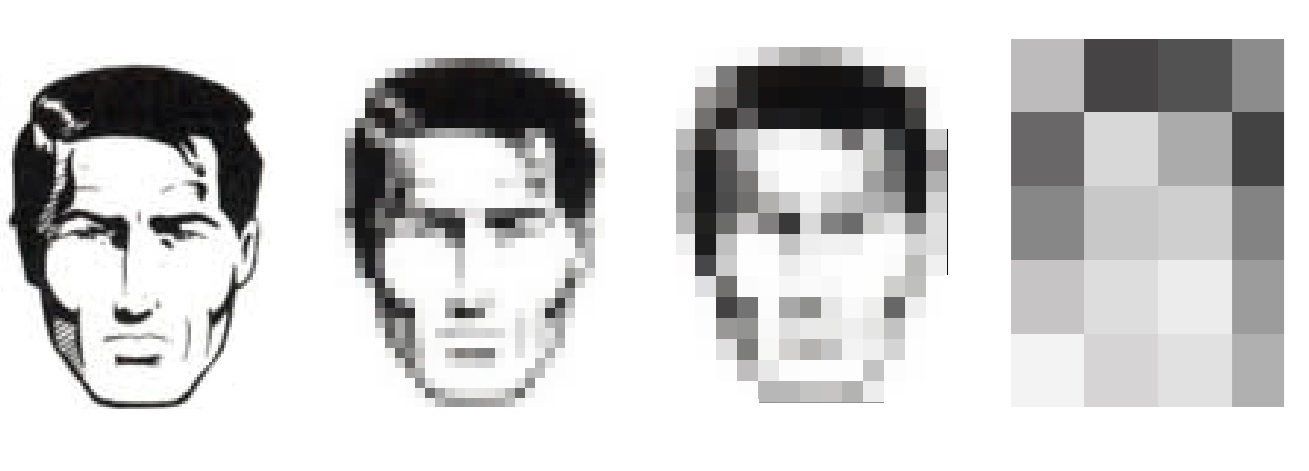
\includegraphics[width=11cm, height=4cm,
		keepaspectratio]{pix.jpg}
		
		{figure 1}
		\\
	\end{center}
  
	
	In figure one from left to right in the first part 
	we can see a drawing of  male face which is already abstraction of the reality but we can easily understand the it’s a human male face even more details about his age and emotional state just from the image , in the second part we also can understand that is the same image that had been pixelated we lose some information but still a human face , the third image we can understand that it looks like  human face without any more information that abstraction make the image more generic but less representative of one face  , in the last image it’s a grid of 5*4 squares of different gray level that is all what we can understand from the image , all of those images generated from the same image the differed is the pixelisation process which been applied throw the pixel art softwear after the pixelisation we will replace every step tail from the subject image with new image from libirary wich have similar RGB value to the tile step from the main image this method called \textbf{\emph{Photomosaics}} .\\
	
	
	\par
	
	Given an image $ I_(x,y) $,change it to rectangular grid of N cells , and dataset of small rectangular images , find N tile images in the dataset and place them in the
	grid such that each cell is covered by a tile that ‘resembles’
	the image portion covered by the tile.
	 \\
	\par
	

\begin{center}
		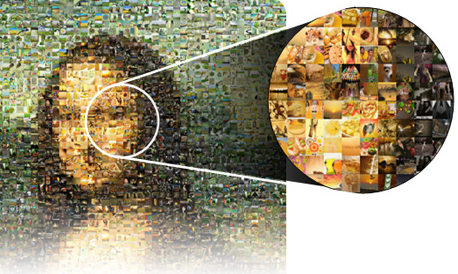
\includegraphics[width=15cm, height=7cm, 
	keepaspectratio]{pixelart2} 
	
	{figure 2}\\
\end{center}

	

		


   \section{History of Photomosaics}
   
  The process of making pictures from other pictures was import part for study the human \emph{Perception } , In 1973 Leon
   Harmon a researcher in mental/neural processing, particularly regarding vision, who worked at Bell Telephone Laboratories he worked on human perception, computer vision and graphics the who study the Photomosaics to understanding some of these in his article "The Recognition of Faces" (Scientific American, November 1973).
    presented a work including several
   “block portraits” . Harmon used these
   “pixelated” portraits to study human perception and the
   automatic pattern recognition issues.
   
   Computer replicated images made from tiled digital
   photographic pictures is recent because it requires large
   computational resources. Robert Silvers began
   working on the first photomosaic while he was a graduate
   student at the MIT Media Lab. Each tile in his images
   represents much more than a single value. Smaller pictures
   match the overall image in tone, texture, shape and color, Silvers subsequently patented the process, founded a company devoted to photomosaics.
  
	
	\chapter{The Methodology}
	
	A mosaic is an image traditionally composed of small pieces of material, such as stone or glass. A photomosaic, on the other hand, is a digital image that made up of other digital images, pieced together by software. Photomosaics are generally credited to Robert Silvers, who developed the technique while he was a student at MIT \cite{Robert}.
	
	How good photomosaics are created is something that has not been formally analyzed, however. For one thing, the idea is relatively new; for another, the quality of a good photomosaic depends in part on properties of the human eye and how we see colors and images , if the tail size from the original subject image is much bigger for example the image lose a lot of detail and would be hard to recognize . 
	the main issues to address in terms of making a soft wear to generate a photomosaics is :-
	\begin{description}
   \item[$\bullet$ ]	How can you define something similar to a minimum color distance between a part of the original picture and a bunch of photos in a library?
	
   \item[$\bullet$ ]	How big can each mosaic be before it loses the details of the original image?
	
   \item[$\bullet$ ]	How many photos should you have in your library?
	
   \item[$\bullet$ ]	How can we rebuild the new photomosaics image ?
   \end{description}

	
	
	The first step was to understand how to find an average color for a picture. We knew, that color pixels are made up of the three color components red, green, and blue (RGB). The combination of different amounts of RGB makes very specific colors , our idea was to take the total sum of each RGB pixel on a photo, then divide the result with the total number of pixels used after the value of the main color computed and entered in a vector(s) .\\
	\begin{center}
		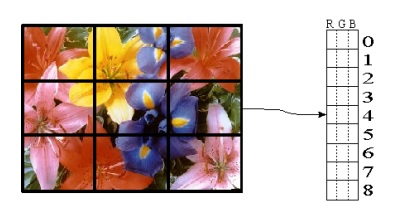
\includegraphics[width=15cm, height=7cm, 
		keepaspectratio]{Untitled}
		{figure 3}
	\end{center}
	 This is done in advance of computing the photomosaic. The vector can be reused for different photomosaics provided for new subject image or new tile set of images , then find out the average color of all images in the library. We then with this information we calculate the Euclidean RGB color distance  of each picture in the image library with the tail cell from the subject image .
	
	Then, for the tile image whose average Rt, Gt, and Bt
	values most closely match it is selected to represent the step pixel in the subject image . The matching is based on
	the Euclidean RGB color distance as follows:
	$$	d(s, t) =  \sqrt{(rs-rt)^2} + \sqrt{(gs-gt)^2}  + \sqrt{(bs-bt)^2} $$
	Here s represents the subject pixel step , t represents the tail image, (rs, gs, bs) are the color values
	of the subject pixel step , and (rt, gt, bt) are the average color values of the tail. \\
	The tile image average with the minimal distance to the subject pixel is the best-matching tail\cite{MIT}.
	
	
	\chapter{Softwear development}
	
		
	\begin{center}
		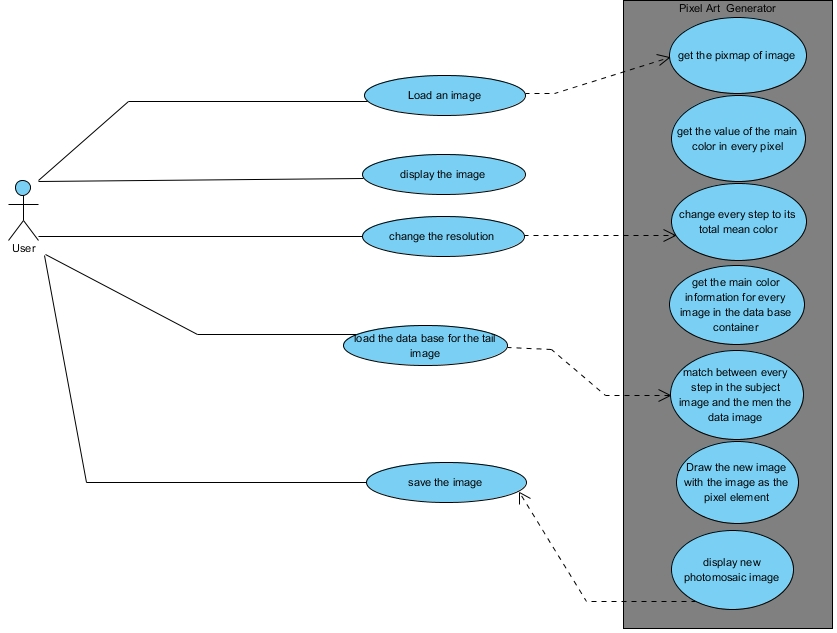
\includegraphics[width=15cm, height=10cm, 
		keepaspectratio]{UseCase} 
		
		{figure 4 -\textbf{Use case Digram}}\\
	\end{center}
	\vspace*{2cm}
	
	
	\section{project objectives}
	


	The project has been divided into several objectives, listed below:
	

	
		\begin{description}
	
	   	\item[$\bullet$ ]Take a photo (source image) to process.
	
 	    \item[$\bullet$ ]Make a grid over this photo.
	
		\item[$\bullet$ ]loop over at every tail on the grid.
		\item[$\bullet$ ] Make library for the main color of every tail in subject image .
	
		\item[$\bullet$ ]Calculate the average color of each tail.
		
		\item[$\bullet$ ] Take a group of images which will be the tail match image .
		
		\item[$\bullet$ ] Make library for the main color of every image in the new group .
	
		\item[$\bullet$ ]	Find the nearest image in the library with the same/near average color of the tail and substitute it in that cell.
	
		\item[$\bullet$ ]	Repeat the process for each tail in the grid.
		\item[$\bullet$ ] Draw the new image 

\end{description}

\section{The Data containers }

The main task in the program is to get RGB value of the subject image and the tail images store them and after apply searching and matching over the stored values and map the matched RGB value to its source in the tail images case or its position - step - in the subject image case , for that we preferred to use Vector as our data container classes , as it is the  most useful container in the C++ standard library , the vector is a convenient, flexible, efficient (in time and space), in our softwear we will use Qvector as part of the QTL\cite{5}  
 
 
 
 \section{Step class}
 
 We will create class as a blue print for or step from the main subject image to represent and save the information of every step from the main image (RGB main color - X position - Y position ) and member functions to get the main color value and access the date member of the class .
 
 \begin{center}
 		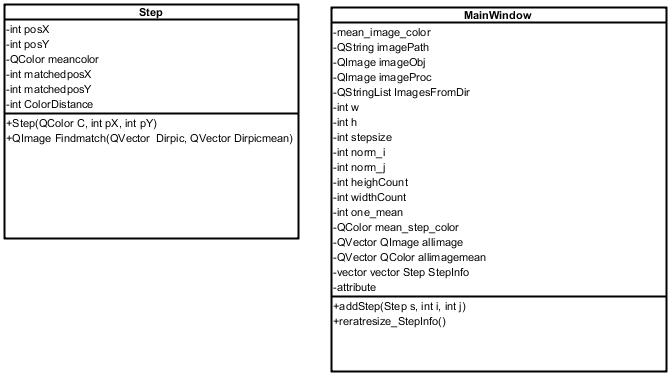
\includegraphics[width=15cm, height=7cm, 
 	keepaspectratio]{Class} 
 	
 	{figure 5 - Class digram}\\
 \end{center}
 
 
 \section{Draw the photomosaics}
 
 For drawing the tail image inside the main subject image we will use \textbf{QPainter Class}\cite{6} and drawImage function 
 
 
 \section{Graphical User Interface }
 
 The GUI is simple as it should be to show the main idea of the project with out complexity 
 
 \begin{center}
 		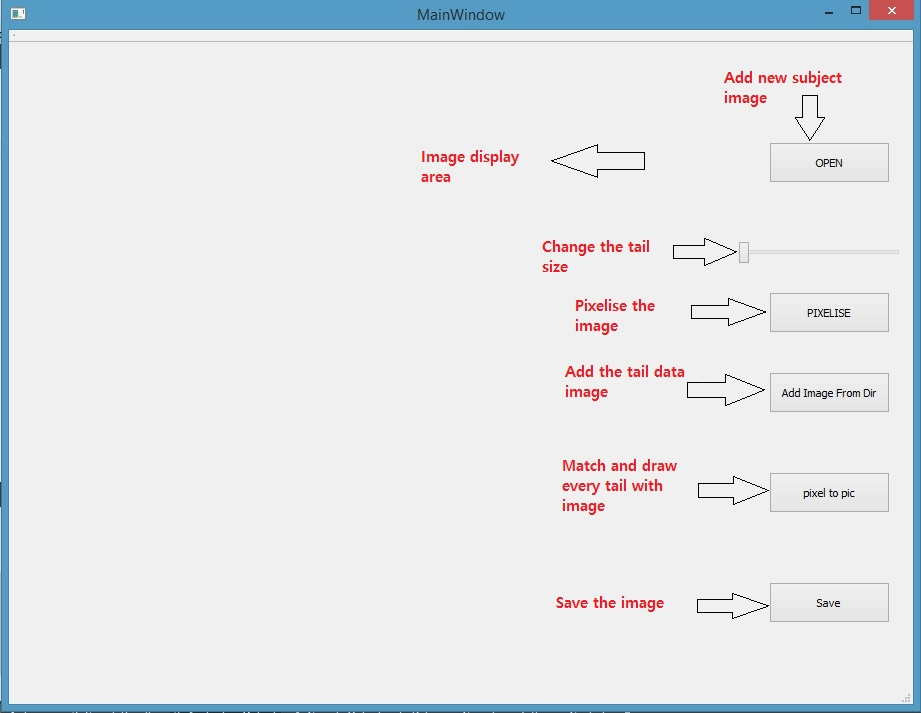
\includegraphics[width=14cm, height=6cm, 
 	keepaspectratio]{mainwindow} 
 	
 	{figure 6 - GUI}\\
 	
 \end{center}
 
 
 
	\chapter{Result }
	
	
	
	\begin{center}
	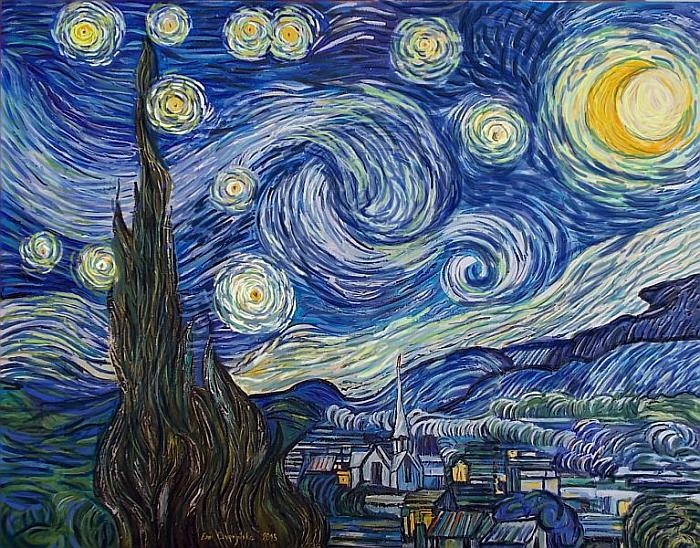
\includegraphics[width=14cm, height=6cm, 
		keepaspectratio]{GN} 
		
		{\textbf{Input Image} - Starry Night by Vincent van Gogh}\\
		
		
	
		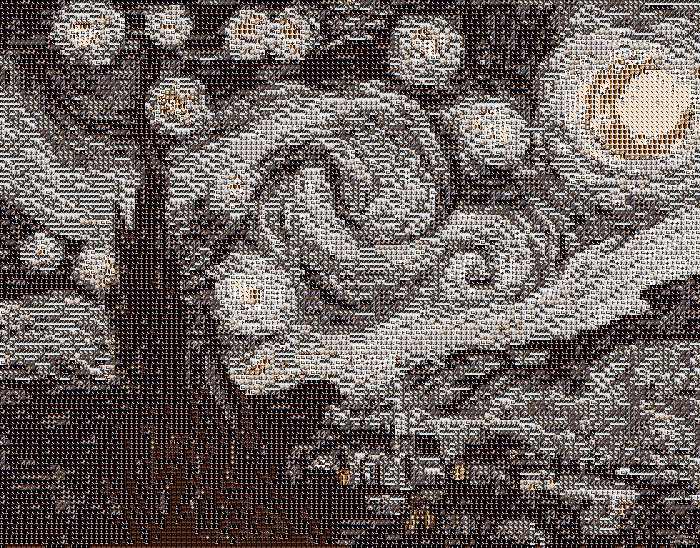
\includegraphics[width=14cm, height=6cm, 
		keepaspectratio]{output-5} 
		
		{output image - Starry Night full of coffee by Vincent van Gogh , Me and Qt step size 5 }\\
		

	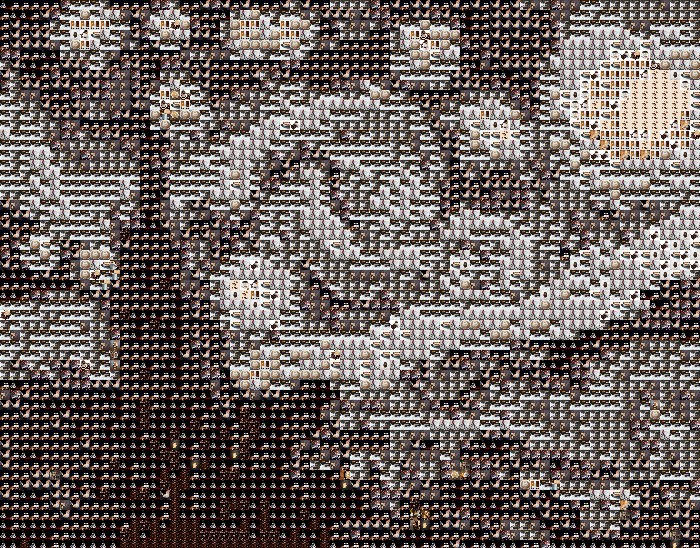
\includegraphics[width=14cm, height=6cm, 
		keepaspectratio]{output-10} 
		
		{output image - Starry Night full of coffee by Vincent van Gogh , Me and Qt step size 10 }\\
		
			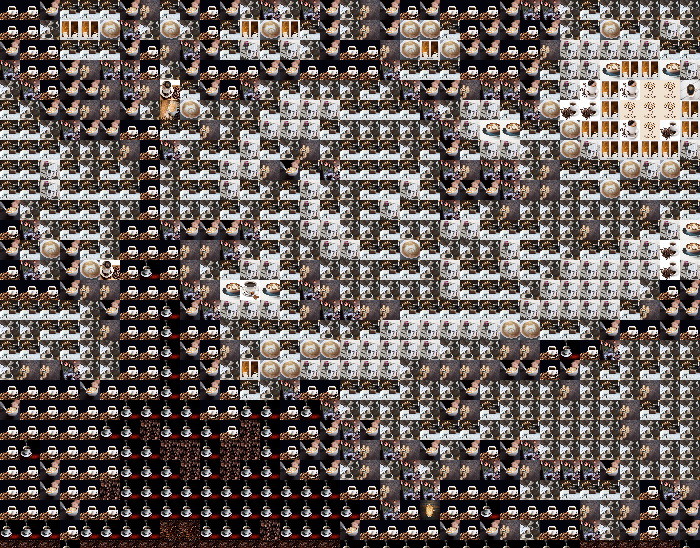
\includegraphics[width=14cm, height=6cm, 
		keepaspectratio]{output-20} 
		
		{output image - Starry Night full of coffee by Vincent van Gogh , Me and Qt step size 20 }\\
		
		
	\end{center}
	
	
	
	\chapter{Future Improvements}

	From the work we had done and the observation if we aim to improve the softwear to find better way to search and match throw the data containers and increase the amount of image in the data containers for the tail match speed up the search process , and also apply different shapes for the tail not just grid of squares , in farther application we can study the Photomosaics  with image segmentation to replace the pixels which is in specific region with image from the data base .

	
	 
	\begin{thebibliography}{9}
		\bibitem{Robert} 
		 Nicholas Tran - Generating Photomosaics: An empirical study.
		\bibitem{MIT}
		An Interdisciplinary Introduction to Image Processing [Steven L. Tanimoto]
		
		\bibitem{1}Digital Mosaic Frameworks - An Overview  [S. Battiato, G. Di Blasi, G. M. Farinella and G. Gallo]
		\bibitem{3}Understanding Photomosaics By Manuel Lopez Michelone and Marcelo Perez Medel.
		
		\bibitem{4} Photomosaic Maps by Filip Jaskolski
		
		\bibitem{5} QTL or STL? - https://web.archive.org/web/20160902015144/http://blog.codeimproved.net/posts/qtl-stl.html
		
		\bibitem{6} http://doc.qt.io/qt-4.8/qpainter.html
		
		
	
	\end{thebibliography}
	
\end{document}
	
